% DO NOT COMPILE THIS FILE DIRECTLY!
% This is included by the other .tex files.

\begin{frame}
\titlepage
\end{frame}

\begin{frame}
  \frametitle{The aim of this presentation}
  \begin{itemize}
     \item A small update on the state of MISP's ongoing development
     \item Some highlights of the changes that were introduced
     \item Upcoming changes
     \item Seperate presentation on Cerebrate
  \end{itemize}
\end{frame}

\begin{frame}
  \frametitle{MISP's evolution since the last MUG}
  \begin{itemize}
    \item Since the last MUG (03/12/2020) we've had:
    \begin{itemize}
        \item 13 releases
        \item 2429 commits
        \item 63 contributors contributing to the core software and its components
    \end{itemize}
  \end{itemize}
\end{frame}

\begin{frame}
  \frametitle{Ramping up the development efforts}
  \begin{itemize}
      \item MISP Professional services has taken off
      \item Fast-tracked support, custom development, private training offerings
      \item Additional funds invested in the development efforts
      \item Growth of the core developer team
      \item Luciano Righetti (@righel) joins the core dev team
      \item Continued herculean effort by Jakub Onderka in improving the internals of MISP
  \end{itemize}
\end{frame}

\begin{frame}
  \frametitle{So what were the main changes?}
  \begin{itemize}
     \item The usual {\bf bug- and usability-fixes, quality of life improvements}
     \item Constant internal refactors to prepare us for moving to a more {\bf modern software stack}
     \item Security fixes, including {\bf several CVEs} (keep your MISP up to date!)
     \item Constantly evolving {\bf context libraries and integrations}
     \item Several major features
  \end{itemize}
\end{frame}

\begin{frame}
\frametitle{OpenAPI documentation}
\begin{itemize}
	\item New, detailed OpenAPI documentation
        \item Integrated directly into MISP with its own visualisation
        \item Broad coverage of all APIs
        \item Parameter examples and explanations
        \item Sample responses along with potential error responses
        \item \url{https://www.misp-project.org/documentation/openapi.html}
\end{itemize}
\end{frame}

\begin{frame}
\frametitle{OpenAPI}
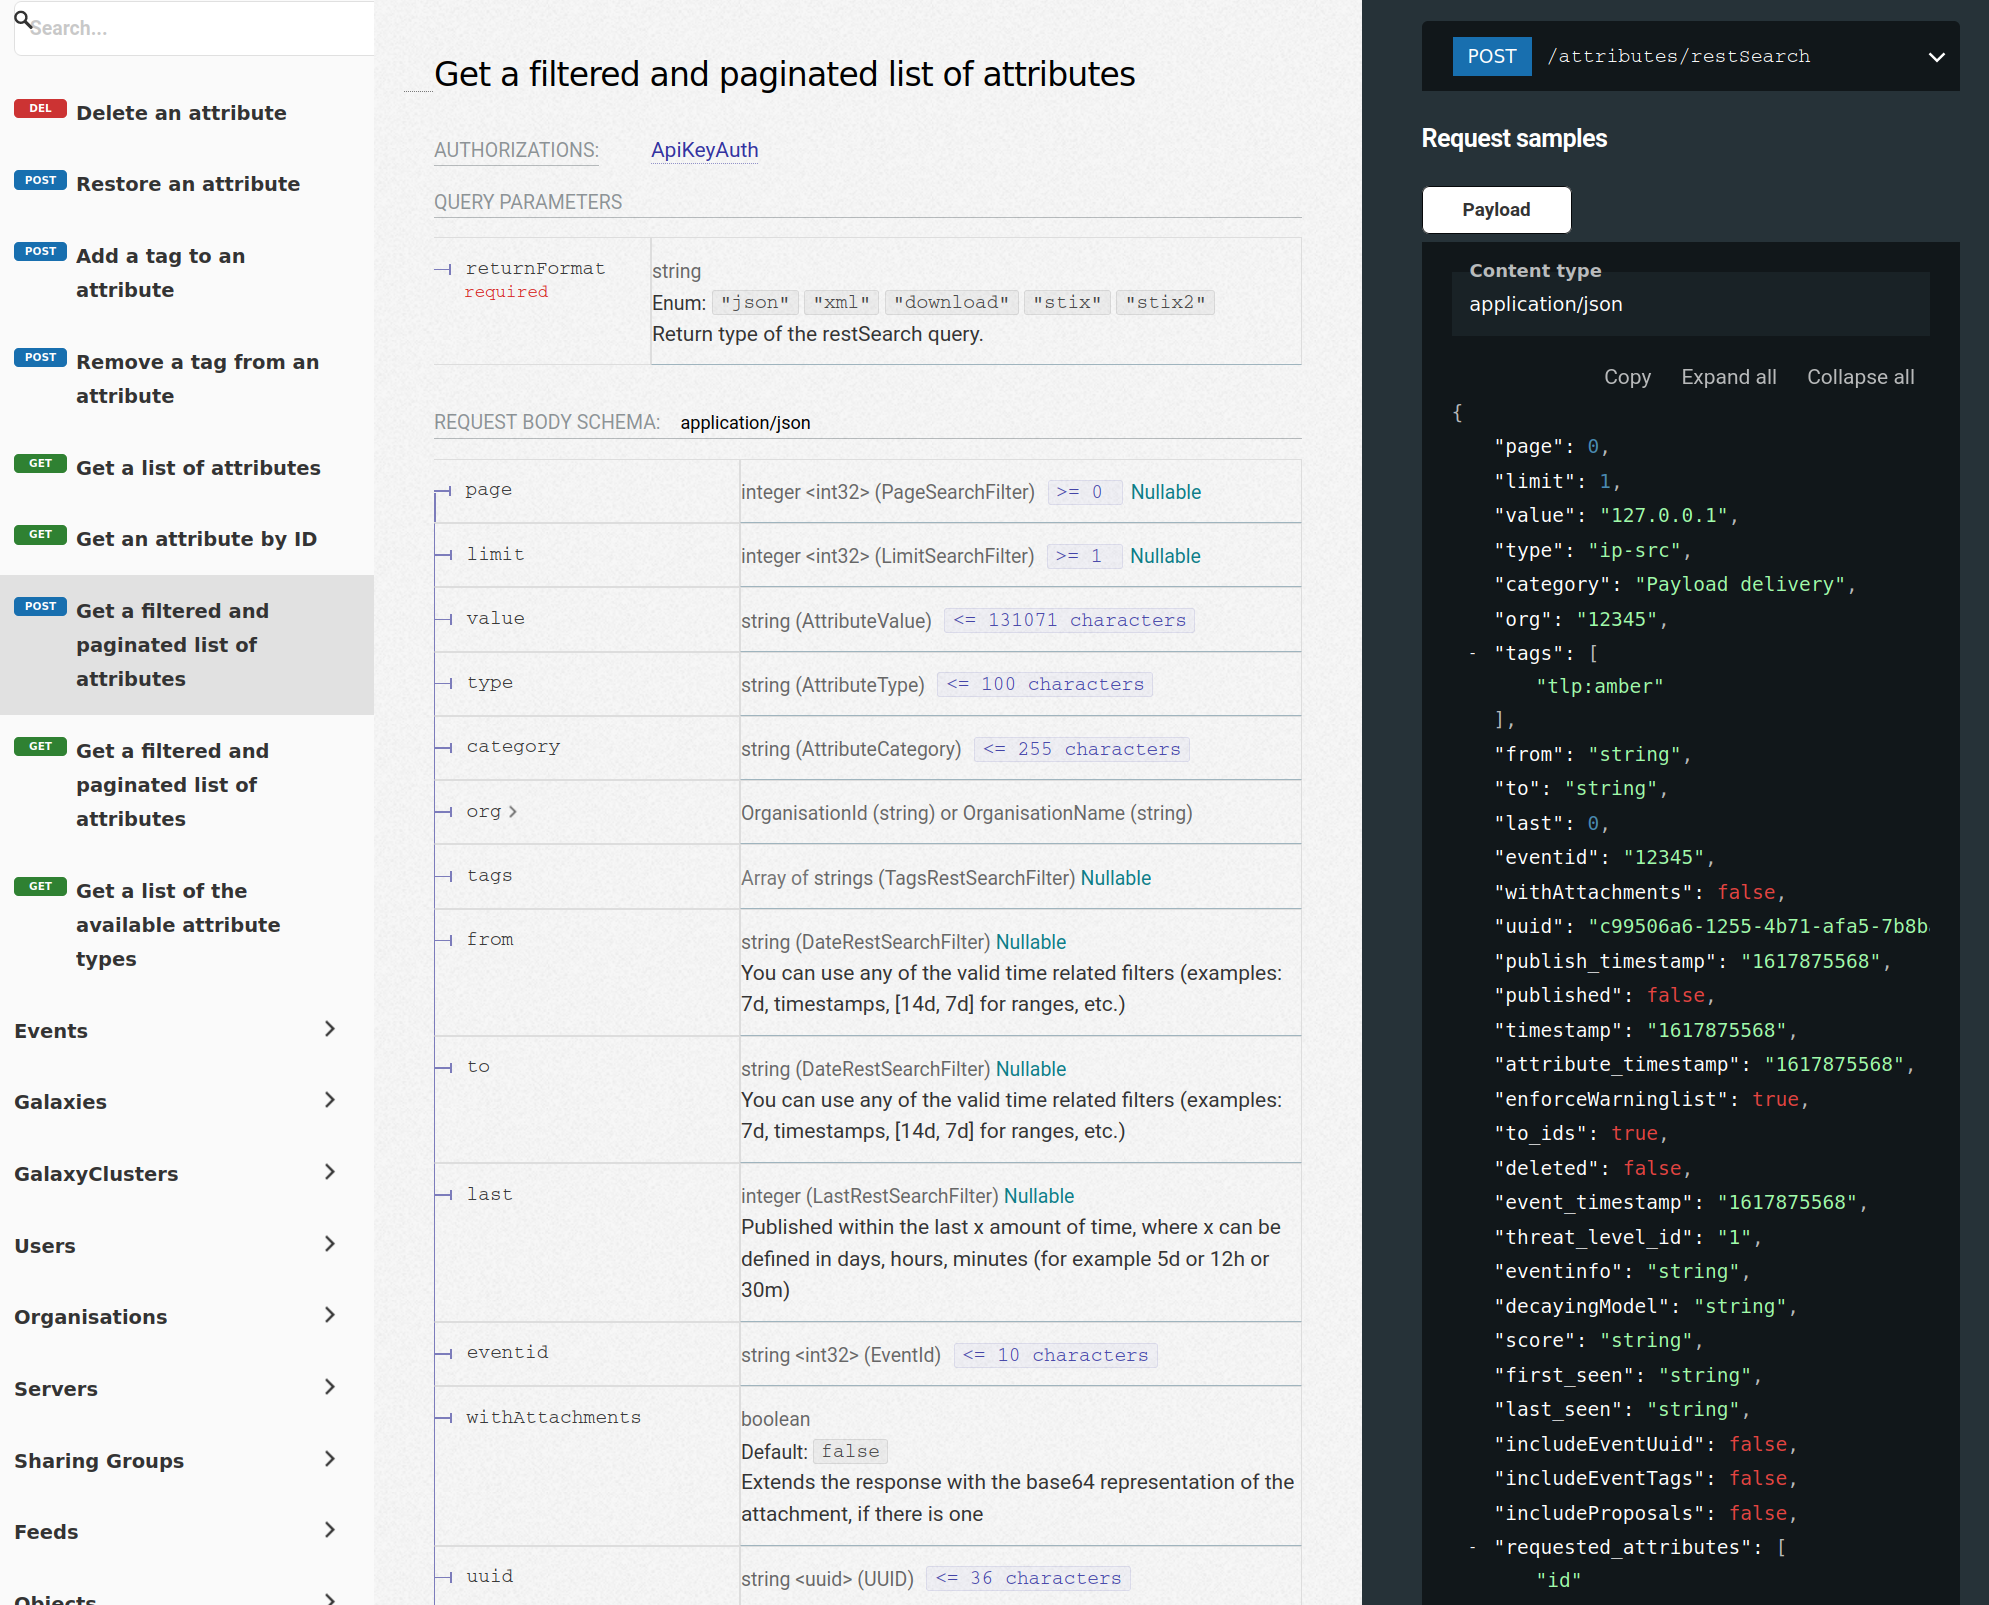
\includegraphics[scale=0.18]{images/openapi.png}
\end{frame}

\begin{frame}
\frametitle{Custom warninglists}
\begin{itemize}
	\item Create warninglists ad-hoc
        \item Add / modify values
        \item {\bf Replaces} the old regex lists for blocking
        \item Use the full potential of the various {\bf matching algorithms}
\end{itemize}
\end{frame}

\begin{frame}
\frametitle{Correlation management}
\begin{itemize}
	\item Constantly being improved
        \item Monitor problematic correlations
        \item Create exclusion rules
\end{itemize}
\end{frame}

\begin{frame}
\frametitle{Authentication}
\begin{itemize}
	\item Documentation of the entire authentication flow
        \item Additional authentication methods supported (OpenID, Azure AD)
        \item Improvements and cleanup of the authentication logic
        \item Various improvements to existing authentication module behaviour
\end{itemize}
\end{frame}

\begin{frame}
\frametitle{Integration}
\begin{itemize}
	\item Rework of the MISP modules system
        \item Support all MISP structures in module data returned (including reports)
        \item Long list of new modules (hashlookup, greynoise, McAfee Mvision, vmware\_nsx, ...)
        \item Direct integration with Cerebrate and CyCat in the MISP core
\end{itemize}
\end{frame}

\begin{frame}
\frametitle{Monitoring and management}
\begin{itemize}
	\item Blog posts on integration with various monitoring tools
        \item New CLI tools to support monitoring efforts
        \item Cerebrate's MISP management functionalities
\end{itemize}
\end{frame}

\begin{frame}
\frametitle{STIX integration complete rework}
\begin{itemize}
	\item After a full year of focused work from Christian Studer (@chrisr3d) the new system is nearly ready
        \item Comprehensive {\bf STIX 1.1.1, 1.2, 2.0, 2.1} support for ingestion and export
        \item Extraction of the MISP-STIX subsystem to a separate {\bf stand-alone library}
        \item Detailed {\bf mapping documentation}
        \item STIX export on the attribute scope in addition to the event scope
        \item \url{https://github.com/MISP/misp-stix}
\end{itemize}
\end{frame}

\begin{frame}
\frametitle{MISP browser extension}
\begin{itemize}
        \item New expansion to {\bf highlight and query data} in MISP(s) from websites
        \item Developed by @MorisotAnselme (during his internship @ CIRCL)
	\item Still in beta, pending the final release
        \item \url{https://github.com/MISP/misp-expansion}
        \item \url{https://addons.mozilla.org/af/firefox/addon/misp-expansion/}
\end{itemize}
\end{frame}

\begin{frame}
\frametitle{Various improvements}
\begin{itemize}
	\item New Dashboard widgets
        \item E-mail notification management
        \item Reworked less usable UI interfaces (such as tag filters)
        \item Object cross-referencing across extended events
        \item Loads of new CLI tools
        \item Refactoring of a large part of the code-base
\end{itemize}
\end{frame}


\begin{frame}
\frametitle{What's in the pipe?}
\begin{itemize}
	\item Further work on the move to the new tech stack
        \item Correlation engine rework
        \item Cryptographic {\bf signing of data}
        \item More flexible distribution model (multiple sharing groups)
        \item New UI
        \item Private Set Intersection (PSI) (allowing correlation sharing/privacy-aware export)
\end{itemize}
\end{frame}

\begin{frame}
\frametitle{Cerebrate}
\begin{itemize}
        \item Last time we've already mentioned that we started working on a {\bf community} and {\bf fleet management} tool
	\item Let's flip to the {\bf Cerebrate} presentation...
\end{itemize}
\end{frame}

\begin{frame}
  \frametitle{To sum it all up...}
  \begin{itemize}
     \item The MISP {\bf developer community} continues to grow and stay active
     \item The main focus this year is on the consolidation of existing functionalities
     \begin{itemize}
          \item Performance, security, UX improvements
          \item Monitoring and large scale management tooling
          \item Fleshing out the documentation and supporting materials
     \end{itemize}
     \item Cerebrate is aiming to fill the void of community/fleet management that we currently have
     \item Definitely no lack of new ideas and improvements, if you want to participate, it's easy to {\bf get involved}
     \item Prioritisation is hard. {\bf Let us know what you think we should focus on}!
  \end{itemize}
\end{frame}

\begin{frame}
  \frametitle{Get in touch if you have any questions}
  \begin{itemize}
    \item Contact CIRCL
    \begin{itemize}
      \item info@circl.lu
      \item \url{https://twitter.com/circl_lu}
      \item \url{https://www.circl.lu/}
    \end{itemize}
    \item Contact MISPProject 
    \begin{itemize}
      \item \url{https://github.com/MISP}
      \item \url{https://gitter.im/MISP/MISP}
      \item \url{https://twitter.com/MISPProject}
    \end{itemize}
    \item Cerebrate project
    \begin{itemize}
      \item \url{https://github.com/cerebrate-project}
      \item \url{https://github.com/cerebrate-project/cerebrate}
    \end{itemize}
    \item Join the COVID-19 MISP community
    \begin{itemize}
      \item \url{https://covid-19.iglocska.eu}
    \end{itemize}
  \end{itemize}
\end{frame}
